\documentclass[fr]{../../../../../../eplexam}

\hypertitle{Théorie et algorithmique des graphes}{5}{INMA}{1691}{2018}{Janvier}{Majeure}
{BAC3 MAP 2018--2019\and Guillaume Funck \and Gilles Peiffer}
{Vincent Blondel et Jean-Charles Delvenne}

Veuillez expliquer vos raisonnements avec clarté,
répondre à des questions différentes sur des feuilles \emph{différentes},
sans oublier d'apposer \emph{votre nom} sur chacune.

\section{Question 1}
Démontrez qu'un graphe est biparti si et seulement si pour tout $k$,
tout sous-graphe induit de $k$ n\oe{}uds
contient un ensemble indépendant de $k/2$ n\oe{}uds ou plus.

On rappelle qu'un sous-graphe induit du graphe $G$
est un sous-graphe construit en choississant un sous-ensemble de n\oe{}uds,
et \emph{toutes} les arêtes reliant ces n\oe{}uds.

\begin{solution}
\begin{proof}
	\noindent
	\newline
	$\boxed{\implies}$
	\newline
	On se convainc facilement que pour tout $k$,
	l'ensemble indépendant induit maximum
	est de taille minimale lorsque l'on choisit $\frac{k}{2}$
	(ou $\frac{k+1}{2}$ et $\frac{k-1}{2}$ si $k$ impair)
	n\oe{}uds dans chaque partition.
	Dès que l'on prend davantage de n\oe{}uds
	dans l'une ou l'autre partition,
	l'ensemble indépendant maximum contiendra
	tous les n\oe{}uds de la partition la plus grande.

	\noindent
	\newline
	$\boxed{\impliedby}$
	\newline
	Procédons par l'absurde.
	Imaginons qu'un tel graphe possède un cycle de longueur impaire.
	Examinons ce cycle comme sous-graphe induit de $G$.
	Comme le cycle est de longueur impaire,
	il possède $\frac{k-1}{2}$ éléments indépendants deux à deux.
	Or $\frac{k-1}{2} \le \frac{k}{2}$,
	nous avons donc une contradiction.
\end{proof}
\end{solution}

\section{Question 2}
Vrai ou faux? Justifiez.

\begin{enumerate}
	\item Il existe un graphe simple à $6$ n\oe{}uds
	dont les degrés sont $1,2,3,3,4,5$.
	\item Le graphe de l'hypercube de dimension $n \ge 1$
	(dont les n\oe{}uds sont les points de coordonnées binaires de $\R^n$
	et les arêtes relient les n\oe{}uds à distance euclidienne unité)
	est planaire si et seulement si $n = 1,2$.
	\item Un arbre de degré maximum $10$ possède au moins $10$ feuilles.
	\item Tout graphe biparti hamiltonien possède un couplage parfait.
	\item Le Rêve du Roi Soleil est possible
	(Sa Majesté souhaitait décorer chaque pièce
	de l'étage noble de Versailles d'or, ou d'argent,
	ou de marbre ou de miroirs---et quand on passait d'une pièce à l'autre,
	le décor devait toujours varier, pour susciter l'émerveillement).
	\item \emph{Bonus}: tout graphe à $m$ arêtes
	possède une coupe à $m/2$ arêtes ou moins.
\end{enumerate}

\begin{solution}
	\begin{enumerate}
		\item Vrai, on sait tracer le graphe.
		\item Faux.
		On peut facilement représenter
		un hypercube de dimension $3$ sur une sphère.
		Par projection stéréographique,
		tout graphe que l'on peut représenter sur une sphère
		sans que ses arêtes ne s'intersectent est planaire.
		\item Vrai.
		Procédons par récurrence.
		Initialisation: Lorsqu'il n'y a qu'un seul n\oe{}ud,
		le degré maximum vaut $1$ et il y a une feuille.
		Induction: admettons que la propriété soit vraie
		pour $\Delta(G) = n-1$.
		Si l'on rajoute un n\oe{}ud
		et qu'on trace une arête vers un n\oe{}ud
		qui n'est pas de degré maximal,
		le graphe possèdera une feuille en plus.
		Si l'on rajoute un n\oe{}ud
		et qu'on trace une arête vers un n\oe{}ud est de degré maximal,
		le graphe possèdera une feuille en plus
		et le degré maximal aura augmenté d'un aussi.
		Nous avons donc
		dans tous les cas $n_{\textnormal{feuilles}} \ge \Delta(G)$.
		\item Vrai.
		Comme le graphe est hamiltonien,
		il possède un cycle qui passe par chaque n\oe{}ud
		une et une seule fois.
		D'autre part, vu qu'il est biparti,
		ce cycle est de longueur paire.
		On peut construire un couplage parfait en suivant ce cycle.
		Un n\oe{}ud sur deux,
		on couple le n\oe{}ud où l'on se trouve avec le suivant.
		\item Vrai.
		Puisque l'étage noble de Versailles
		peut être représenté comme un graphe planaire,
		il y a toujours moyen
		de colorier chaque face (chaque pièce) dans une couleur
		(or, argent, marbre ou miroir).
		\item Faux.
		Contre-exemple: prenons le graphe complet à trois n\oe{}uds.
		Sa coupe minimale est de taille $\Delta(G) = 2$,
		or $2 \ge \frac{3}{2}$.
	\end{enumerate}
\end{solution}

\section{Question 3}
Napoléon Bonaparte campe près d'Austerlitz, avec ses six généraux.
À la veille du $2$ décembre 1805,
ils désirent se mettre d'accord sur le protocole de communcation
lors de la bataille décisive.
Chaque général (y compris Napoléon) garde auprès de lui six messagers
pour communiquer avec les six autres généraux, il y a donc 42 messagers.
Le temps en minutes que le messager met
pour joindre chaque paire de généraux est indiqué dans la table ci-dessous.

L'Empereur se rend compte que vu l'efficacité variable des messagers
il est parfois plus rapide de passer par un ou plusieurs généraux intermédiares
pour en atteindre un autre.
Il demande à l'officier du génie que vous êtes
de calculer la stratégie de communication la plus rapide
pour qu'Il puisse communiquer ses ordres à chacun de ses généraux.

\begin{enumerate}
	\item Combien de minutes lui faut-il pour joindre Bessières?
	Bernadotte? Davout? Soult? Lannes? Murat?
	Représentez le graphe des généraux
	(les n\oe{}uds) et des messagers (les arêtes)
	utilisés dans votre stratégie.
	\item Combien de messagers, devenant inutiles dans votre stratégie,
	peuvent rejoindre le champ de bataille?
	\item Conseillez-vous à l'Empereur d'implémenter cette stratégie?
\end{enumerate}

\begin{table}[H]
	\centering
	\begin{tabular}{c|ccccccc}
		& Napoléon & Bessières & Bernadotte & Davout & Soult & Lannes & Murat \\
		\hline
		Napoléon & 0 & 21 & 13 & 5 & 13 & 24 & 20 \\
		Bessières & 21 & 0 & 12 & 10 & 10 & 5 & 7 \\
		Bernadotte & 13 & 12 & 0 & 7 & 7 & 12 & 10 \\
		Davout & 5 & 10 & 7 & 0 & 9 & 19 & 17 \\
		Soult & 13 & 10 & 7 & 9 & 0 & 9 & 9 \\
		Lannes & 24 & 5 & 12 & 19 & 9 & 0 & 14 \\
		Murat & 20 & 7 & 10 & 17 & 9 & 14 & 0
	\end{tabular}
\end{table}

\begin{solution}
\begin{enumerate}
	\item L'algorithme de Dijkstra nous permet de calculer
	le temps minimum qui sépare Napoléon de ses autres généraux.
	En l'appliquant sur ce problème
	on obtient les temps suivant entre eux:
	\begin{table}[H]
		\centering
		\begin{tabular}{c|cccccc}
		& Bessières & Bernadotte & Davout & Soult & Lannes & Murat \\
		\hline
		Napoléon & 15 & 12 & 5 & 13 & 20 & 20
		\end{tabular}
	\end{table}

	Avec le graphe suivant:

	\begin{figure}[H]
		\centering
		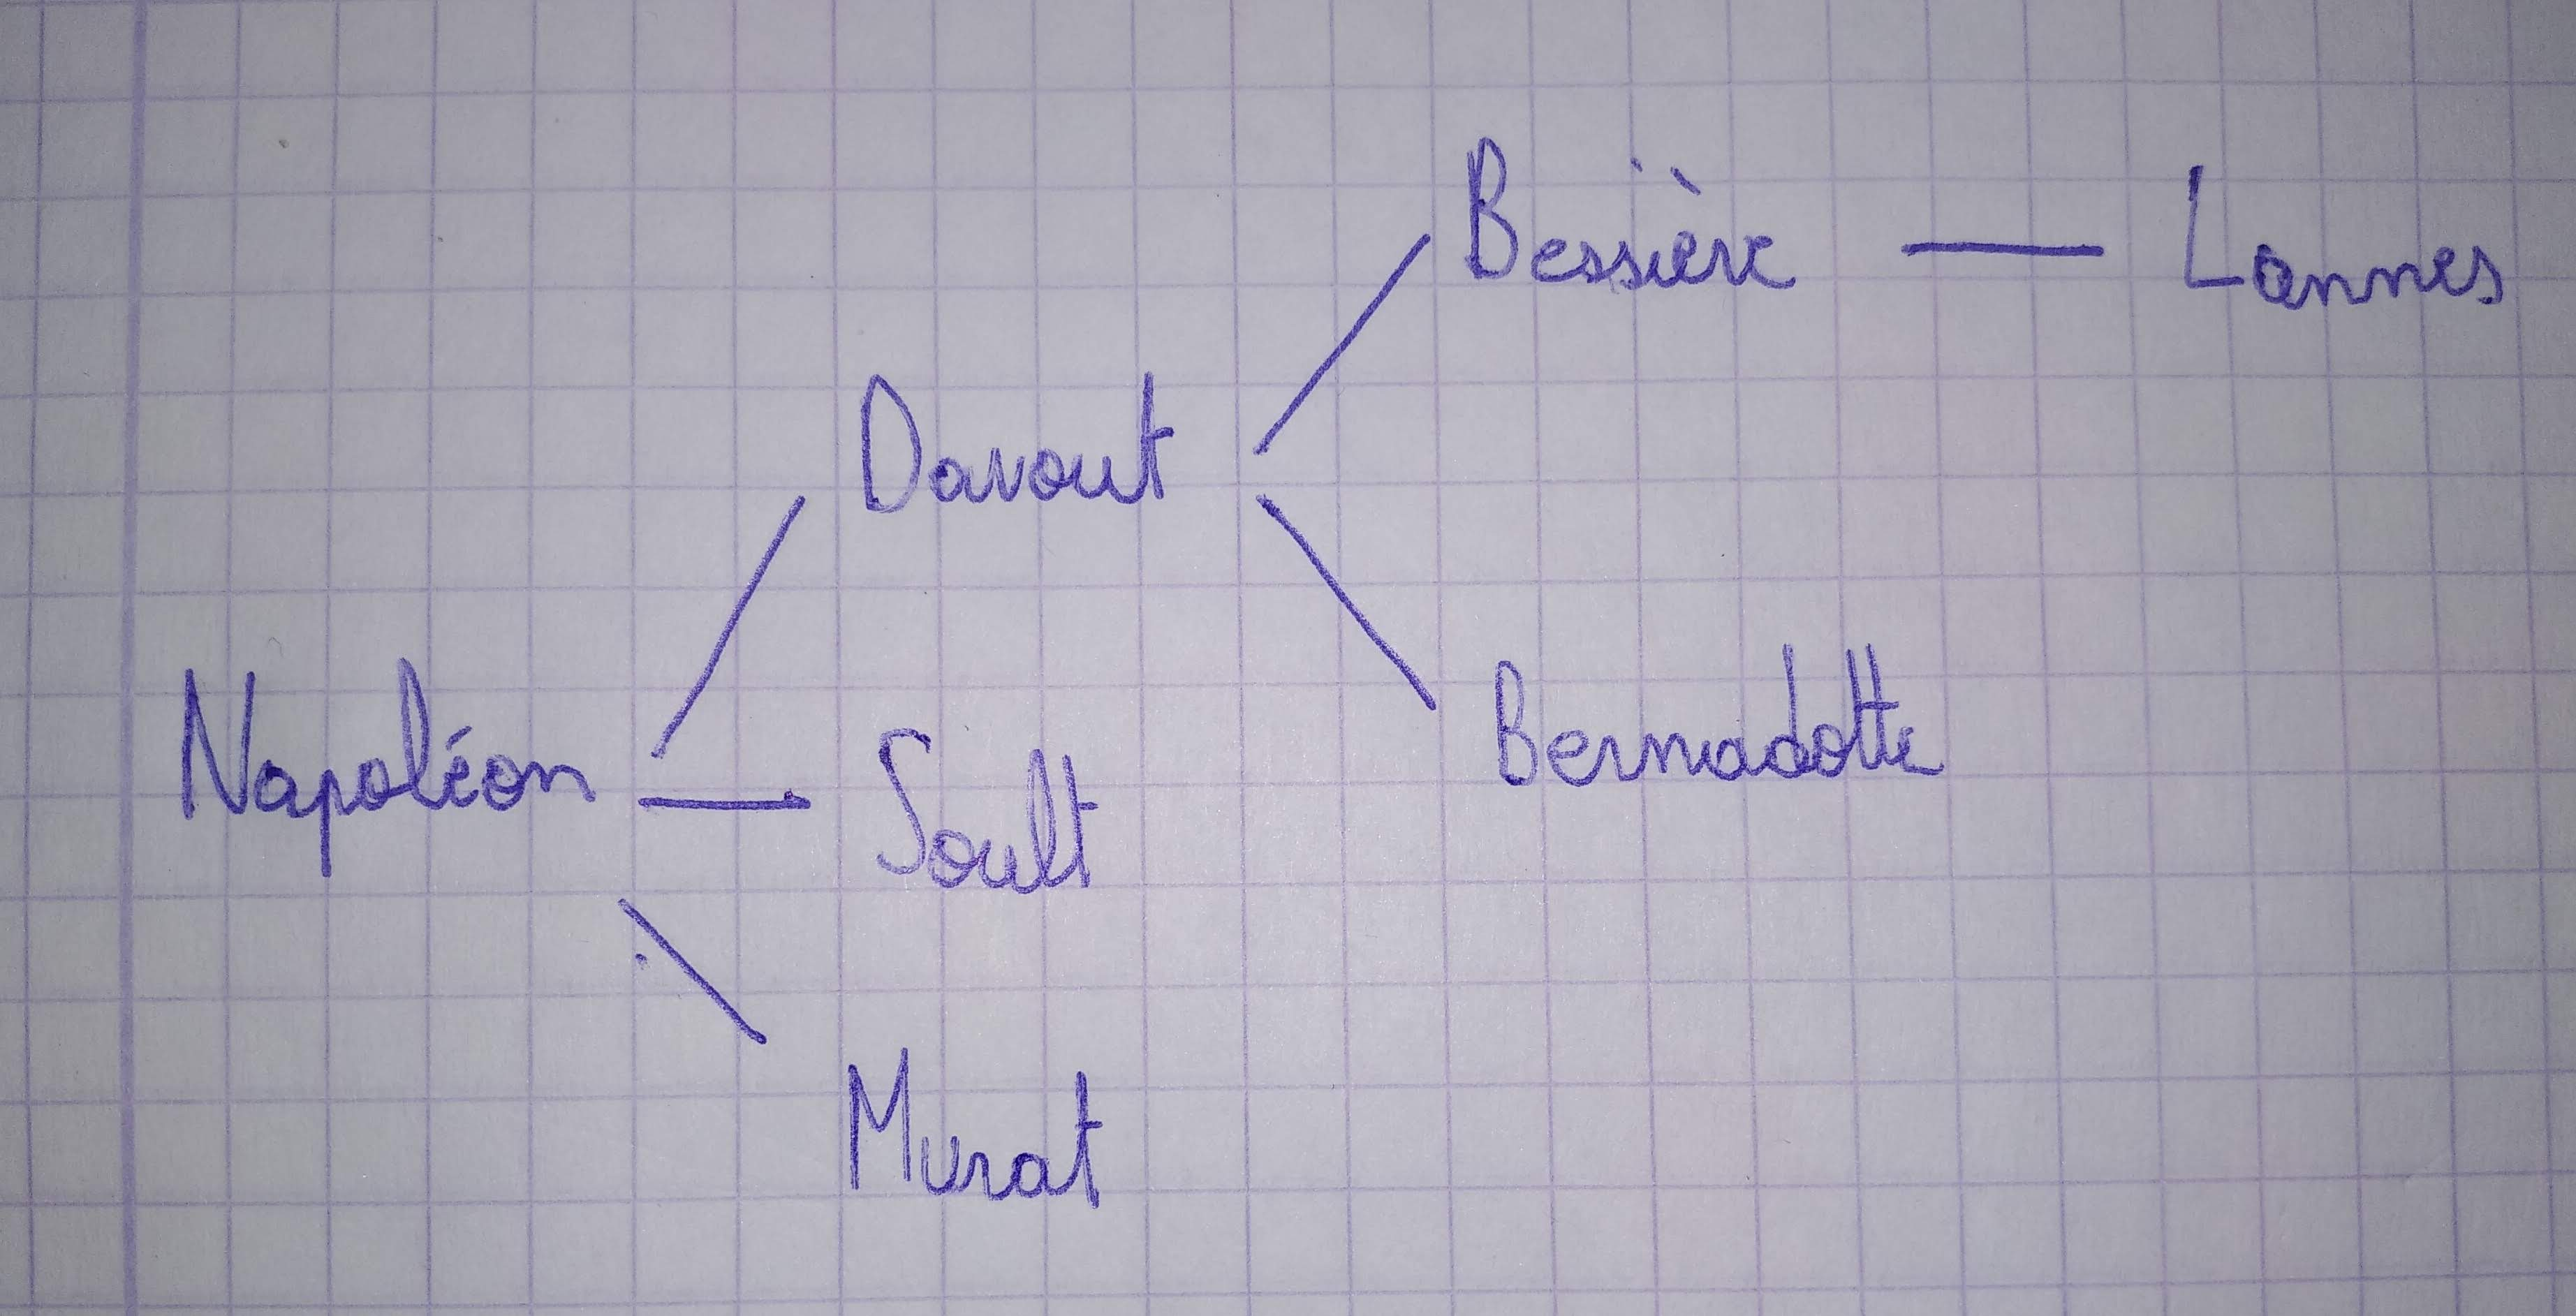
\includegraphics[width=0.7\textwidth]{img/graph.jpg}
	\end{figure}

	\item En utilisant la stratégie vue plus haut,
	on peut se permettre de ne garder que les six messagers
	les plus utiles et donc congédier les $36$ restants.

	\item Non.
	Il faut cependant garder à l'esprit
	que le tableau ci-dessus ne fournit que les distances les plus courtes
	entre Napoléon et ses généraux et pas entre les généraux entre eux.
	On pourrait effectuer l'algorithme de Dijkstra
	en partant à chaque fois d'un nouveau n\oe{}ud
	jusqu'à ce qu'on obtienne un graphe contenant seulement
	les chemins les plus efficaces entre chaque personnage.
\end{enumerate}
\end{solution}

\section{Question 4}
Voici un algorithme dû à Fleury, dans les années 1880,
pour découvrir un parcours eulérien fermé dans les graphe eulériens.

Étant donné un graphe eulérien $G$,
on choisit un n\oe{}ud de départ arbitraire $x_0$.
On choisit une arête pour continuer le parcours et arriver au n\oe{}ud $x_1$.
À chaque étape $t = 0, 1, 2, \ldots$,
le parcours ainsi constitué entre $x_0$ et $x_t$
est prolongé d'une arête
parmi les arêtes non encore visitées incidentes à $x_t$.
La nouvelle extrémité est nommée $x_{t+1}$.
Si on a plusieurs arêtes disponsibles pour prolonger le parcours,
on en choisit une
qui n'est pas un pont dans le graphe des arêtes non encore visitées
(on verra que c'est toujours possible).
On termine si toutes les arêtes du n\oe{}ud $x_t$ ont déjà été visitées.
Le parcours ainsi construit s'avère être un parcours eulérien fermé,
comme on va le montrer.

Par \emph{pont}, on veut dire une arête de coupe,
une arête qui sépare sa composante connexe en deux si on la retire du graphe
(dans ce cas-ci le graphe étant celui des arêtes non encore visitées).

\begin{enumerate}
	\item Démontrez que dans tout graphe avec un parcours eulérien
	(ouvert ou fermé),
	une coupe d'arêtes minimale (pour l'inclusion)
	est de taille impaire si elle sépare les extrémités du parcours
	et de taille paire sinon.
	\item Démontrez que sauf à la toute dernière étape,
	le graphe des arêtes non encore visitées a
	exactement zéro ou deux n\oe{}uds de degrés impairs, $x_0$ et $x_t$.
	\item Démontrez qu'à la dernière étape,
	$x_t = x_0$ et le parcours est fermé.
	\item Démontrez qu'à toute étape de l'algorithme,
	si on a le choix entre plusieurs arêtes (non encore visitées)
	pour prolonger le parcours, au moins une n'est pas un pont.
	\item Démontrez qu'à toute étape de l'algorithme,
	le graphe des arêtes non encore visitées est un graphe connexe,
	plus éventuellement des n\oe{}uds isolés.
	\item Démontrez que le parcours construit par l'algorithme
	visite toutes les arêtes.
\end{enumerate}

L'ensemble de ces étapes prouve bien la correction de l'algorithme de Fleury.

\begin{solution}
\begin{enumerate}
	\item \label{p1} Un parcours eulérien est un parcours
	qui passe par toutes les arêtes d'un graphe.
	Si une coupe sépare les deux extrémités du parcours,
	en partant d'une des deux extrémités,
	le parcours doit bien croiser une première fois la coupe.
	Si le parcours repasse du côté initial de la coupe via une arête,
	elle doit forcément avoir une arête complémentaire
	qui nous ramène de l'autre côté de la coupe.
	La coupe possède donc un nombre impair d'arêtes.

	Dans l'autre cas, on se ramène au cas précédent sauf qu'à la fin,
	le parcours doit retourner une dernière fois du côté initial.
	La coupe possède donc un nombre pair d'arêtes.
	\item On prouve cela par récurrence.
	Au départ, comme $G$ est un graphe eulérien,
	tous les n\oe{}uds du graphe des arêtes non encore visitées
	(que l'on appellera GNV) ont un degré pair.
	En visitant la première arête à partir de $x_0$,
	$x_0$ et $x_1$ perdent tous les deux un degré dans GNV
	et ils deviennent de degré impair.

	Ensuite, on considère que GNV en $t>0$ possède deux n\oe{}uds impairs.
	Lorsque l'on visite une nouvelle arête à partir de $x_t$
	(vers $x_{t+1} \ne x_0$),
	ce dernier n\oe{}ud et $x_{t+1}$
	(qui était de degré pair dans GNV selon notre hypothèse)
	perdent un degré dans GNV
	puisque l'on retire l'arête entre $x_t$ et $x_{t+1}$.
	$x_t$ devient de degré pair et $x_{t+1}$ de degré impair.
	Si $x_{t+1} = x_0$ alors ce n\oe{}ud perd toujours un degré
	mais il devient pair.
	Il y a alors zéro n\oe{}uds de degré impair.
	Pour l'étape suivante, on se retrouve dans le même cas
	que pour la visite de la première arête entre $x_0$ et $x_1$
	et le graphe retrouve deux n\oe{}uds impairs.
	Il y a donc toujours deux ou zéro n\oe{}uds de degré impair.

	\item Quand il ne reste plus qu'une seule arête,
	on sait par le résultat précédent
	que c'est celle entre $x_0$ et $x_t$.
	En effet, un graphe avec deux n\oe{}uds et une arête
	possède deux n\oe{}uds de degré impair, ce sont donc $x_0$ et $x_t$.

	\item Un pont est une arête qui sépare sa composante connexe en deux
	si on la retire.
	C'est donc une coupe impaire (de taille un).
	Par le résultat du point~\ref{p1},
	on sait que dans tout graphe avec un parcours eulérien,
	une coupe d’arêtes minimale est de taille impaire
	si elle sépare les extrémités du parcours.
	Dans notre cas, un pont est forcément une coupe minimale.
	L'autre extrémité du parcours eulérien qu'on recherche dans GNV
	se trouve alors de l'autre côté du pont.
	Puisque l'on sait que notre GNV admet un parcours eulérien
	(il possède zéro ou deux n\oe{}uds de degré impair),
	ce parcours doit passer par toutes les arêtes du côté $x_t$ du pont
	avant de passer de l'autre côté.
	Il y a forcément une arête adjacente à $x_t$ qui n'est pas un pont,
	à moins que $x_t$ soit le seul point de l'autre côté du pont.
	Dans ce cas, on laissera un noeud isolé derrière nous.

	\item Notre graphe initial $G$ est connexe.
	À chaque étape, on supprime une arête de GNV
	mais on a prouvé au point précédent que celle-ci
	n'est pas un pont ou bien un pont relié à un seul n\oe{}ud
	(qui laisserait un n\oe{}ud isolé si on le supprimait).
	À l'exception de ces n\oe{}uds isolés,
	on ne déconnecte donc jamais GNV.

	\item Puisqu'à chaque étape, on ne déconnecte pas le graphe
	(à l'exception des n\oe{}uds isolés)
	et qu'à la dernière étape, $x_0 = x_t$,
	on est obligé de visiter chaque arête de $G$
	avant de revenir à $x_0$ où l'algorithme s'arrête.
\end{enumerate}
\end{solution}
\end{document}
